\subsection{Document Inspections}

A number of documents were collected from the school, relating to both how the quizzes are currently set, and the management structure of the school; these will aid in creating the best possible solution that fits the needs of the school.

\subsubsection{Weekly Email} % (fold)
\label{ssub:weekly_email}
\begin{figure}[h!]
  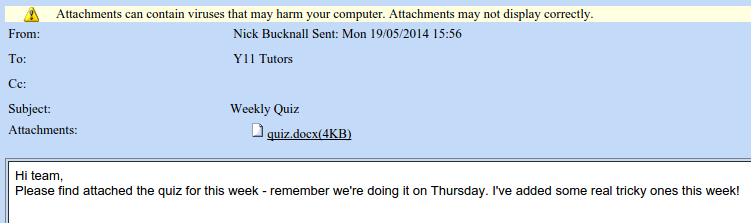
\includegraphics[scale=0.46]{analysis/current_solution/document_inspections/email}
  \caption{Email sent by Nick Bucknall on the 19th May 2014}
\end{figure}

This capture of an email sent by Nick Bucknall (a head of year, soon to be head of house) to his tutor team demonstrates the inefficiency with which the quiz system is currently handled. Sending an email with an attachment once a week is an approach fraught with issues, the most glaring of which is the shocking lack of organisation. As can be gleaned from the shot, the school's email system is not the most modern, and this can make it difficult to find particular emails - such as the weekly quiz. A far better solution would be to have the correct quiz appear automatically.
\clearpage
% subsubsection weekly_email (end)

\subsubsection{Weekly Quiz} % (fold)
\label{ssub:weekly_quiz}
\begin{figure}[h!]
  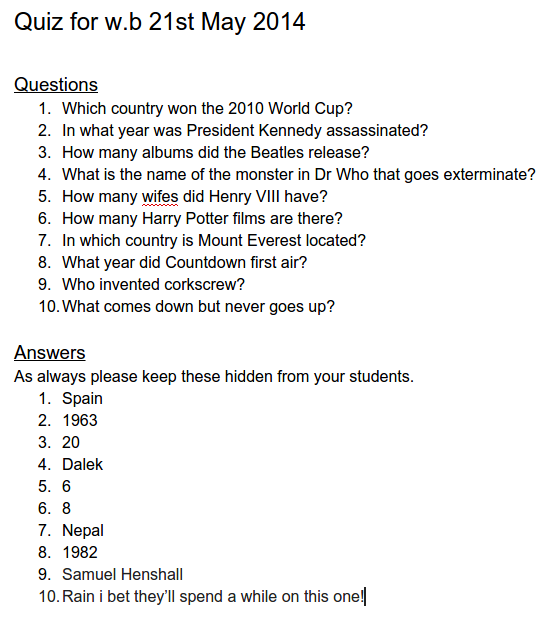
\includegraphics[scale=0.55]{analysis/current_solution/document_inspections/quiz_sample}
  \caption{Quiz created by Nick Bucknall on the 14th May 2014}
\end{figure}

The above capture of a quiz created by Nick Bucknall, and distributed to form tutors, demonstrates the form that that the quizzes currently take. As can be discerned, though the current method undoubtedly works, the existence of the answers so close to the questions causes a number of difficulties; most notably, it means that the questions must be read out by the form tutor, and the actual question sheet cannot be shown. Additionally, it no doubt takes time for Nick Bucknall to lay out the document in such a manner each week; a better solution would be if a standard template could be used (though not, it should be noted, in the form of another word processed document).
\clearpage
% subsubsection weekly_quiz (end)

